\section{Experiments}\label{sec:exp}

Experiments here.

%\begin{figure}[!t]
%\centering
%\begin{tabular}{cc}
%\subfloat[A* nodes: all 140 experiments]{\includegraphics[scale=0.32]{img/tnode_Astar.pdf}} 
%   & \subfloat[RBFS nodes: all 140 experiments]{\includegraphics[scale=0.32]{./img/tnode_RBFS.pdf}}\\
%\subfloat[A* average searched nodes]{\includegraphics[scale=0.32]{./img/anode_Astar.pdf}} 
%   & \subfloat[RBFS average searched nodes]{\includegraphics[scale=0.32]{./img/anode_RBFS.pdf}}\\
%%\subfloat[E]{\includegraphics[width=2cm]{logo}} 
%%   & \subfloat[F]{\includegraphics[width=3cm]{logo}}\\
%\end{tabular}
%\caption{Plots for the number of nodes searched against the problem size for each algorithm and heuristic. For the first 2 figures, for each number of disks 4 to 10, every 20 examples have the same problem size.  We show the average number of expanded nodes against the number of disks for a clear demonstration. As the problem size becomes larger, the number of searched nodes grows exponentially.}
%\label{fig:nodes}
%\end{figure}
%
%\begin{figure}[!t]
%\centering
%\begin{tabular}{cc}
%\subfloat[A*: average cpu time (s) on heuristics]{\includegraphics[scale=0.32]{./img/AHcpu-aver.pdf}} 
%   & \subfloat[RBFS: average cpu time (s) on heuristics]{\includegraphics[scale=0.32]{./img/RHcpu-aver.pdf}}\\
%\subfloat[A*: average cpu time (s) on whole problem]{\includegraphics[scale=0.32]{./img/ATcpu-aver.pdf}} 
%   & \subfloat[RBFS: average cpu time (s) on whole problem]{\includegraphics[scale=0.32]{./img/RTcpu-aver.pdf}}\\
%%\subfloat[E]{\includegraphics[width=2cm]{logo}} 
%%   & \subfloat[F]{\includegraphics[width=3cm]{logo}}\\
%\end{tabular}
%\caption{Plots for the average cpu time against the problem size over 20 examples for each algorithm and heuristic.}
%\label{fig:cputime}
%\end{figure}
%
%\begin{figure}[!t]
%\centering
%\begin{tabular}{cc}
%\subfloat[Nodes against disks for admissible heurisitic]{\includegraphics[scale=0.32]{./img/node_Astar_RBFS_H_ad.pdf}} 
%   & \subfloat[Nodes against disks for non-admissible heurisitic]{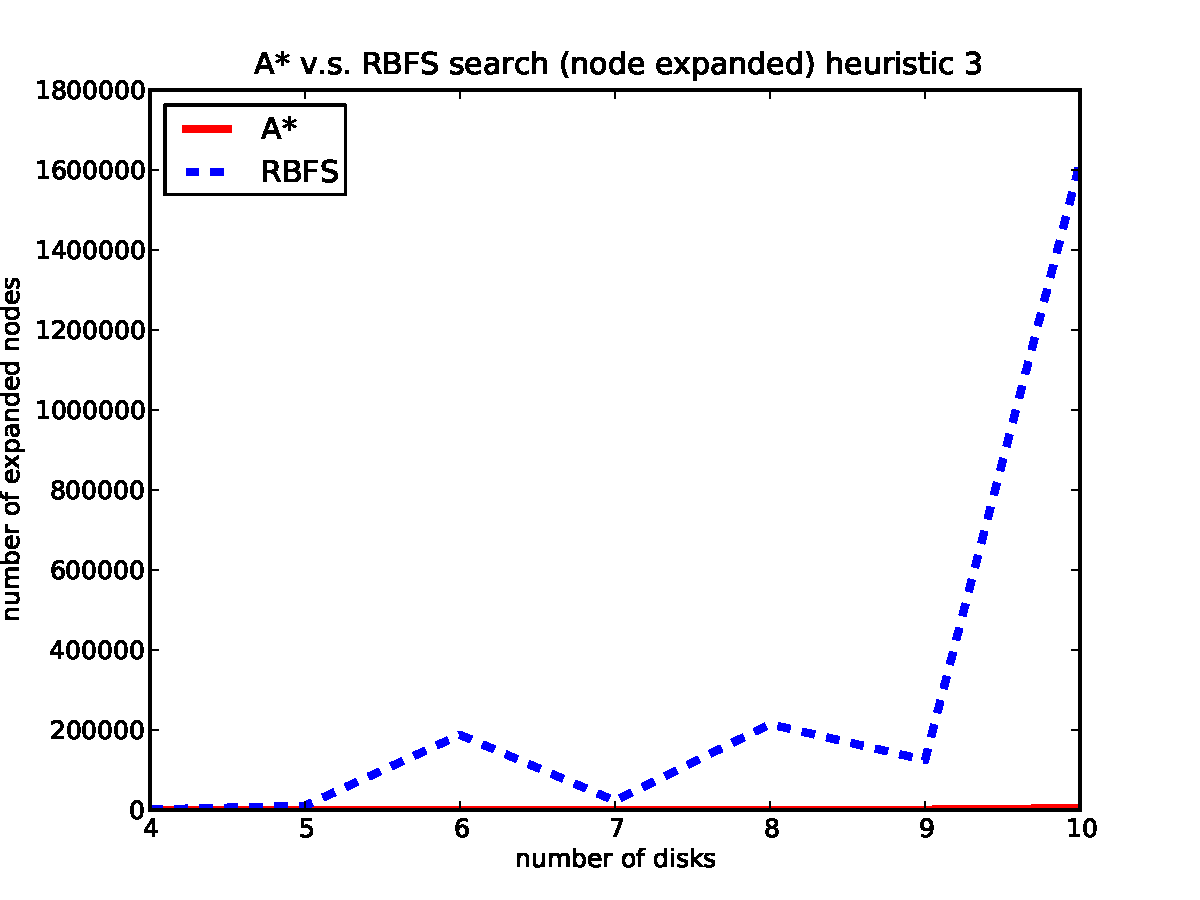
\includegraphics[scale=0.32]{./img/node_Astar_RBFS_H_nad.pdf}}\\
%%\subfloat[cpu time against disks for heurisitic 1]{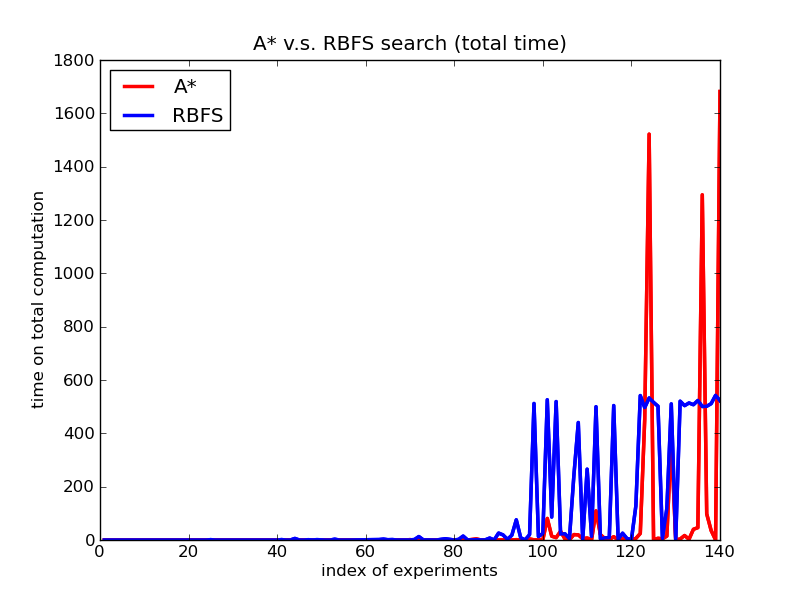
\includegraphics[scale=0.32]{../results/Astar_RBFS_H1_cpu.png}} 
%   %& \subfloat[cpu time against disks for heurisitic 2]{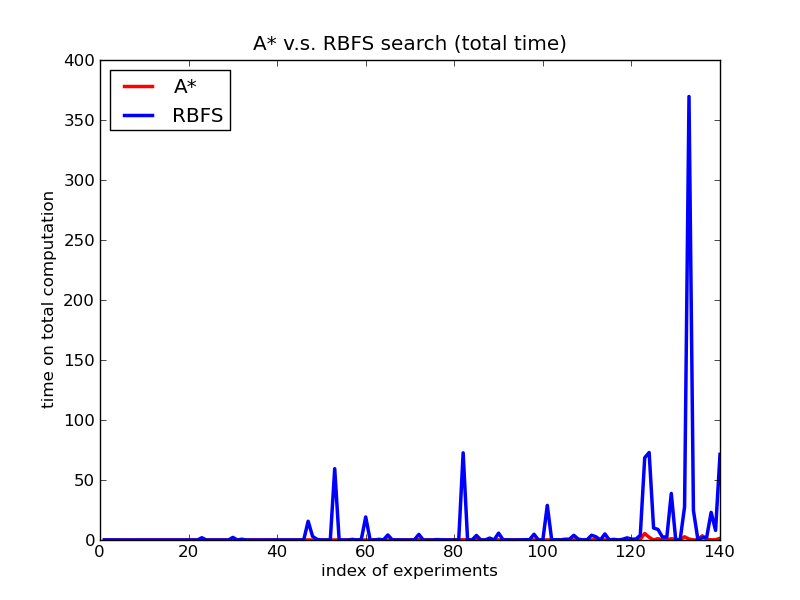
\includegraphics[scale=0.32]{../results/Astar_RBFS_H2_cpu.png}}\\
%\end{tabular}
%\caption{Performance comparisons between A* and RBFS}
%\label{fig:astar-rbfs}
%\end{figure}
%
%\begin{table}[!h]
%    \centering
%    \scalebox{0.9}{
%	    \begin{tabular}{|l|c|c|c|c|c|c|c|}
%		\hline
%		Disks: & 4 & 5 & 6 & 7 & 8 & 9 & 10\\ \hline
%		A*/admissible & 8.8 & 11.6 & 13.95 & 16.5 & 18.6 & n/a & n/a\\ \hline
%		%A*/admissible H7 & 8.95 & 11.6 & 13.95 & 16.75 & 19.2 & 22.4 & 24.77\\ \hline
%		RBFS/admissible & 8.8 & 11.6 & 13.95 & 16.35 & 17.11 & n/a & n/a\\ \hline
%		A*/nonadmissible 1 & 8.85 & 11.85 & 14.6 & 17.5 & 20.2 & 24.1 & 27.6\\ \hline
%		RBFS/nonadmissible 1 & 8.85 & 11.85 & 15.25 & 19 & 22.21 & 26.81 & 32.25 \\ \hline
%		A*/nonadmissible 2 & 9.25 & 12.95 & 16.5 & 20.05 & 23.8 & 27.4 & 34.05\\ \hline
%		RBFS/nonadmissible 2 & 11.25 & 17.85 & 24.35 & 32.75 & 40.35 & 50.7 & 64.55\\ \hline
%	    \end{tabular}
%    }
%    \caption{Average solution length per algorithm, heuristic and disk size. n/a means unable to compute within 10 minutes for all problems. Note that some experiments failed for completing before NMAX nodes; these were not included in the average.}\label{tab:solen}
%\end{table}
